\documentclass[11pt]{article}
\usepackage{style}

\begin{document}

% =============================
% Header
% =============================
\begin{minipage}[t]{0.65\textwidth}
  \hspace{-21pt}
  {\Huge \MyNameCN}

  \vspace{1em}
  \hspace{-20pt}
  邮箱:\MyEmail 

  \hspace{-20pt}
	电话:\MyPhone 

  \hspace{-20pt}
	GitHub:\href{\MyGitHub}{\MyGitHub}

  \hspace{-20pt}
	个人网站:\href{\MyWebsite}{\MyWebsite}
\end{minipage}
\hspace{42pt}
\begin{minipage}[t]{0.2\textwidth}
  \vspace{-35pt} % ensures alignment at top
  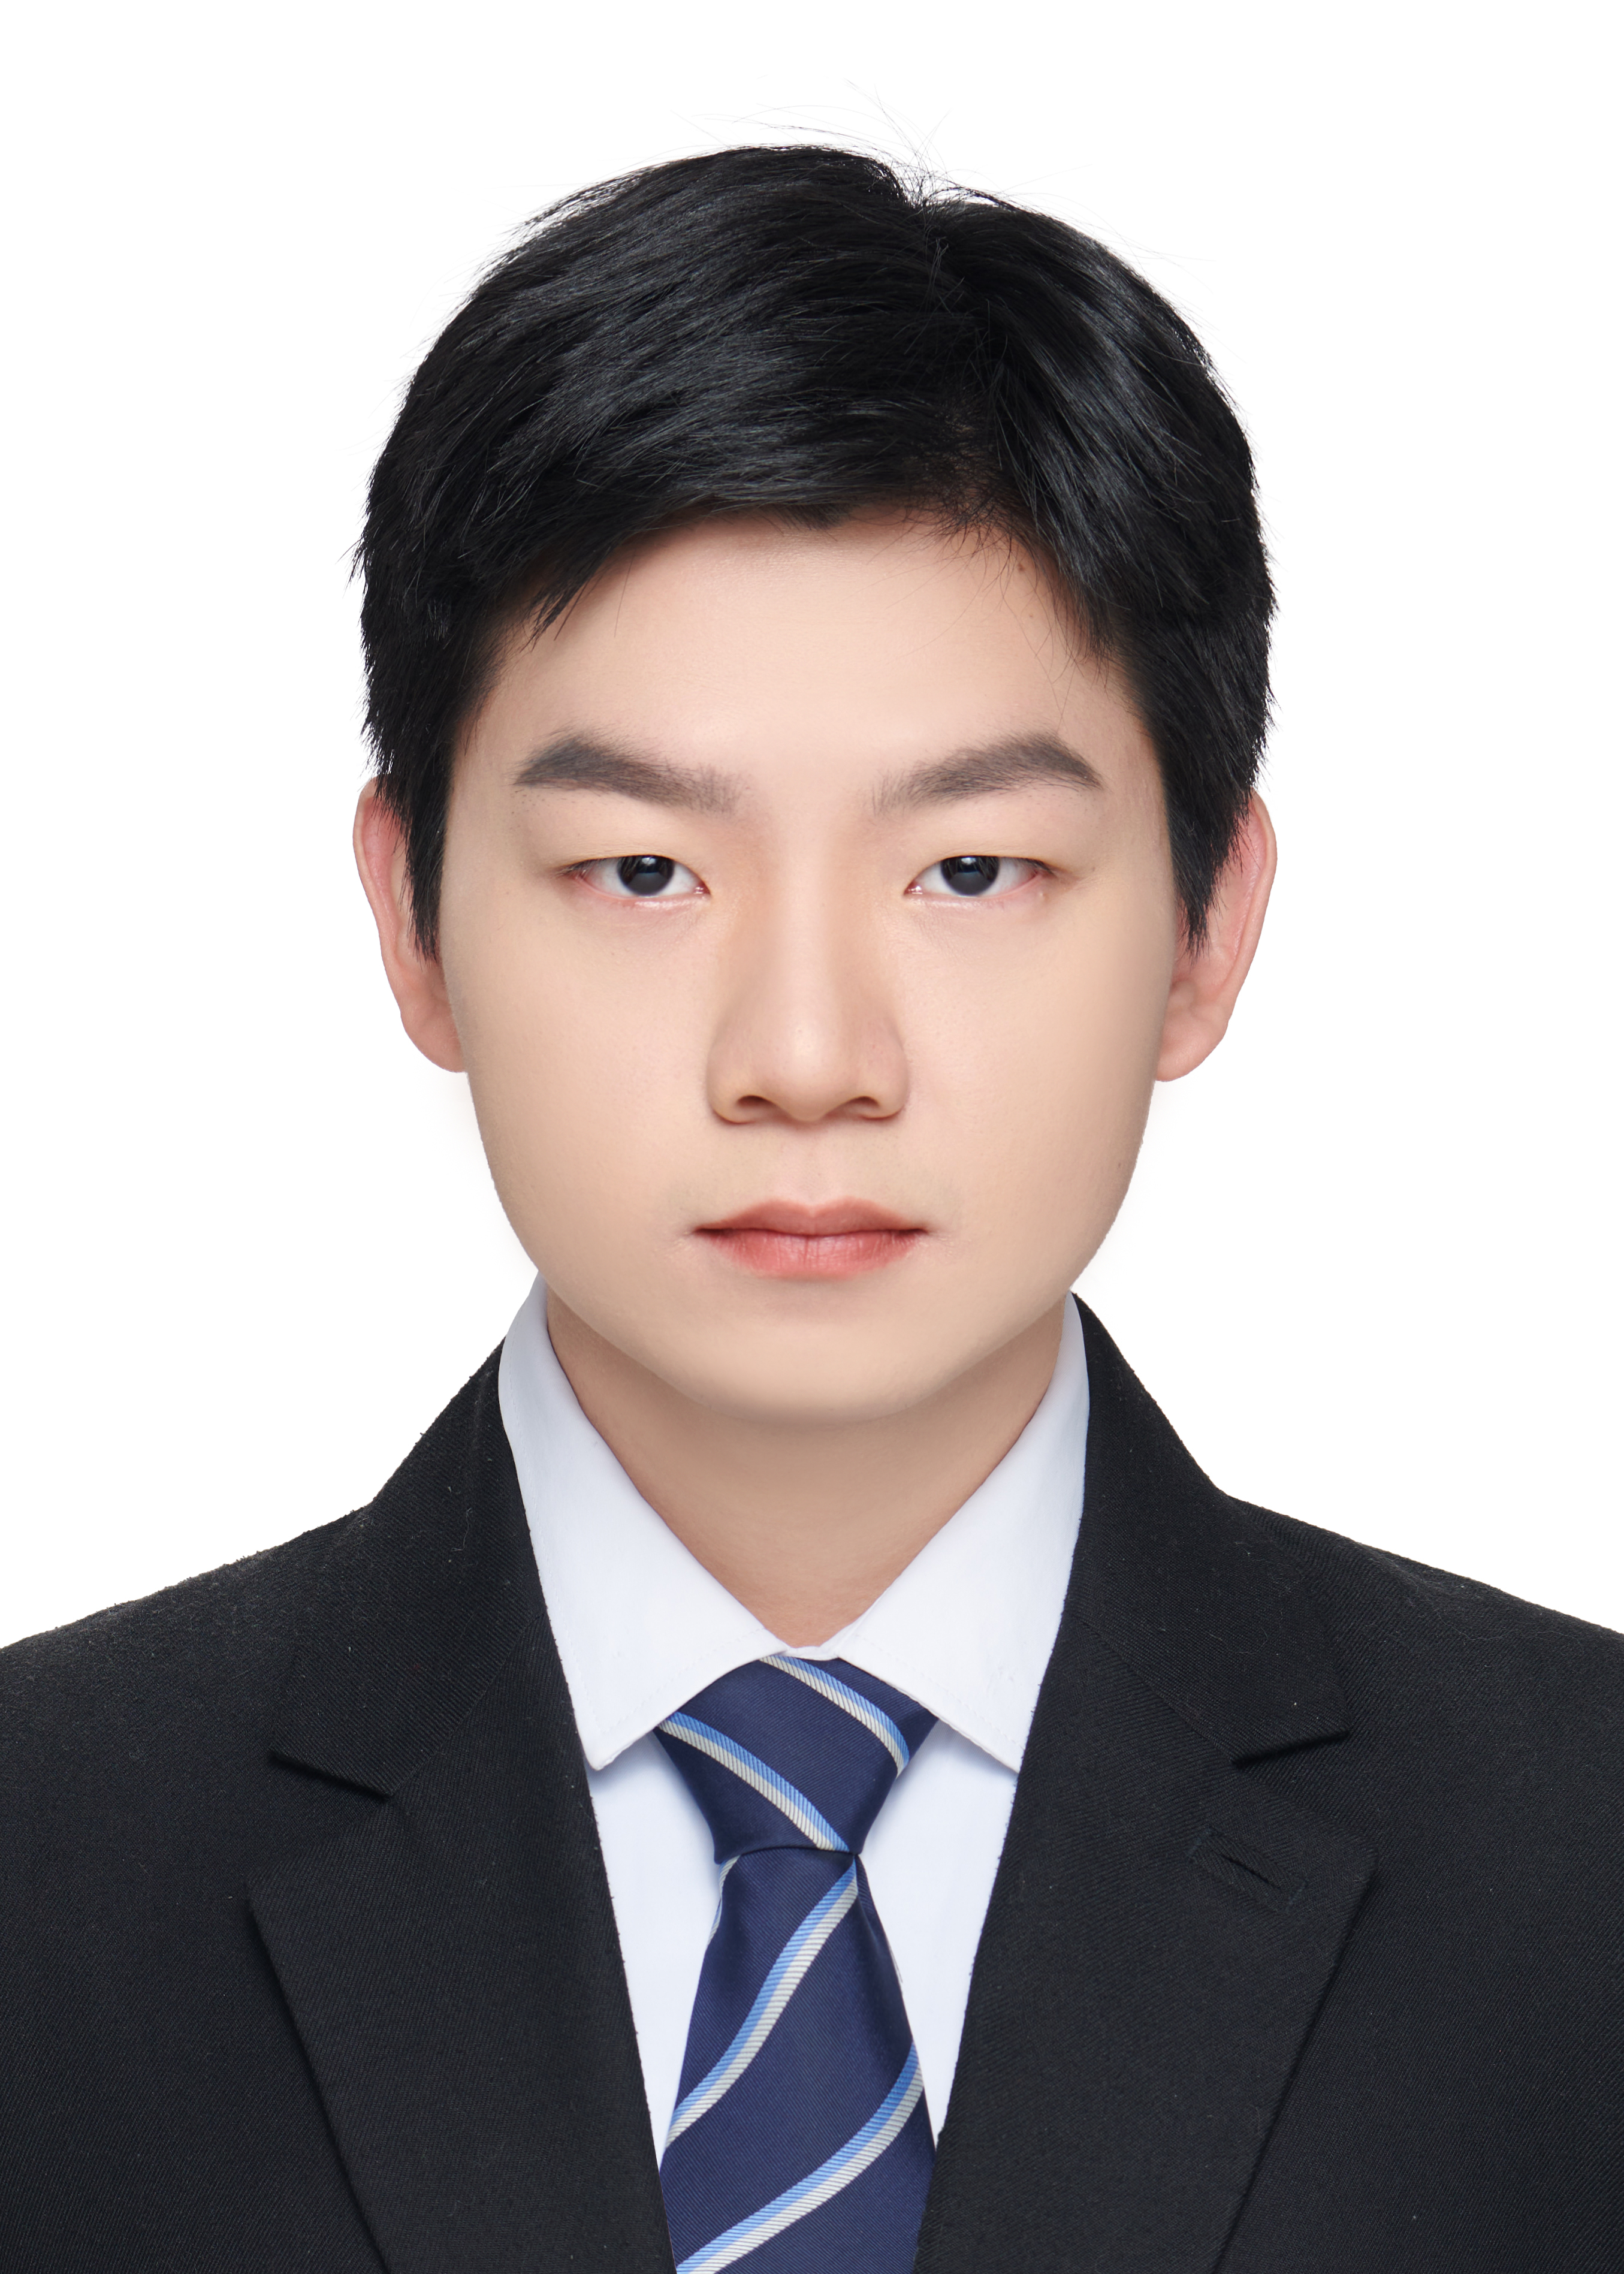
\includegraphics[width=\textwidth]{./images/profile.jpg} 
\end{minipage}
\hfill

\vspace{1em}


% =============================
% Education
% =============================
\CVSection{教育背景}
\EducationEntryCN{悉尼大学 University of Sydney}{2021年2月 -- 2025年11月}
{高级计算机学士 Bachelor of Advanced Computing}{计算机科学}

\EducationEntryCN{悉尼大学 University of Sydney}{2021年2月 -- 2025年11月}
{商科学士 Bachelor of Commerce}{金融}


% =============================
% Publications
% =============================
\CVSection{发表文章}
\PublicationEntry{Stability-Driven CNN Training with Lyapunov-Based Dynamic Learning Rate}{ADC 2024}
{\underline{Tang, D.}, Yang, N., Deng, Y., Zhang, Y., Sani, A.S., Yuan, D.}

\PublicationEntry{Adaptformer: An Adaptive Multimodel Deep Decomposition Approach for Power Consumption Forecasting}{ADMA 2024}
{Yang, N., Zhang, Y., Wang, Y., \underline{Tang, D.}, Li, Y., Yuan, D.}


% =============================
% Work Experience
% =============================
\CVSection{工作经历}
\ExperienceEntryCN{悉尼大学}{2024年 8月 -- 现在}
{计算机学院学术助教}
{\\
ISYS2120 Data and Information Management (2024 S2) \\
}

\ExperienceEntryCN{悉尼大学}{2024年 11月 -- 现在}
{生命与环境学院助理研究员}
{在David James Lab帮助完成 ProteHome 项目开发}

\vspace{2em} % Make the header of Projects show at the top of the next page


% =============================
% Projects
% =============================
\CVSection{项目经历}
\ExperienceEntryCN{ProteHome}{2024年 7月 -- 现在}
{研究助理员、网站开发}{参与网站重构,技术栈包括 Next.js, Django, PostgreSQL, Tailwind;完成全栈开发。}

\ExperienceEntryCN{ioulia.ai}{2024年 1月 -- 2024年 7月}
{联合创始人}{设计技术路线,制定商业计划,完成 MVP 开发,使用 Chain of Thoughts 优化产品效果。}

\ExperienceEntryCN{GigHero}{2023年 4月 -- 2024年 8月}
{联合创始人}{设计技术栈 React, Express, PostgreSQL, Tailwind;完成 MVP 平台开发。}

\ExperienceEntryCN{Searten}{2023年 8月 -- 2023年 11月}
{大学项目,项目经理,全栈开发}{带领团队完成基于 Next.js 和 Tailwind 的 MVP 平台开发。}

\ExperienceEntryCN{学生管理平台}{2022年}
{网站开发}{使用 Django 开发全栈学生管理平台。}

\ExperienceEntryCN{基于 FUSE 的 File System}{2022年}
{大学项目}{C语言开发,实现支持大文件与大文件夹的文件系统。}

\ExperienceEntryCN{操作系统 Scheduler}{2022年}
{大学项目}{C语言开发设计基于 Round Robin 和 MLFQ 的操作系统 Scheduler。}

\end{document}
